\documentclass{article}
\usepackage{url}
\usepackage{color}
\usepackage{multirow}
\usepackage{listings}
\usepackage{float}
\usepackage{amsfonts}
\usepackage{amssymb}
\usepackage{amsmath}
\usepackage{cite}
\usepackage{listings}
\usepackage{xcolor}
\usepackage{graphicx}
\usepackage{draftwatermark}
\usepackage{extarrows}
\SetWatermarkText{DRAFT POST}
\SetWatermarkScale{3}

\lstset{ 
  language=Python,                     % the language of the code
  basicstyle=\footnotesize,       % the size of the fonts that are used for the code
  numbers=none,                   % where to put the line-numbers
  backgroundcolor=\color{white},  % choose the background color. You must add \usepackage{color}
  showspaces=false,               % show spaces adding particular underscores
  showstringspaces=false,         % underline spaces within strings
  showtabs=false,                 % show tabs within strings adding particular underscores
  tabsize=2,                      % sets default tabsize to 2 spaces
  breaklines=true,                % sets automatic line breaking
  keywordstyle=\color{blue},      % keyword style
  commentstyle=\color{darkgray},   % comment style
  stringstyle=\color{black},      % string literal style
} 
\setlength\parskip{.5\baselineskip}
\author{Ryan J. Kung \\ryankung@ieee.org\\}
\title{A Survey of Algebraic Effect System}
\begin{document}
\maketitle
% \tableofcontents

\section{Introduction}

Algebraic effects are an approach to computational effects based on a premise that impure behaviour arises from a set of operations such as get and set for mutable store, read and print for interactive input and output, or raise for exceptions. This naturally gives rise to handlers not only of exceptions, but of any other effect, yielding a novel concept that, amongst others, can capture stream redirection, backtracking, co-operative multi-threading, and delimited continuations\cite{intro-algebraic-effects-and-handlers}.

\subsection{Syntax and Terms}
\begin{figure}[H]
  \centering
  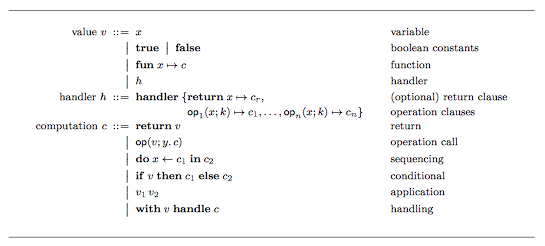
\includegraphics[width=1\linewidth]{src/syntax.png}
  \caption{Syntax of Terms \cite{intro-algebraic-effects-and-handlers}}
\end{figure}

Syntax $do$ is quiet similar to the $do$ of Monad which is present for Sequencing, and the operation calls, it can be considered as a lazy functional call like $v.c := op(x)$. The intro paper\cite{intro-algebraic-effects-and-handlers} give out definition of Generic effect as:

\begin{gather}
  op \xlongequal[]{def} fun\ x \rightarrow op(x; y.return\ y)
\end{gather}

\subsection{Basic Example}

Consider a simple handler is:

\begin{gather}
  getUserName \xlongequal[]{def} fun\ x \rightarrow readline(\_; k) \rightarrow k.promot\ s)
\end{gather}

And this simple input \& output example can be implemented with Python and Effect Library\cite{python-effect}:

\begin{lstlisting}[language=Python]
class ReadLine(object):
    def __init__(self, prompt):
        self.prompt = prompt

def get_user_name():
    return Effect(ReadLine("Enter a candy> "))

@sync_performer
def perform_read_line(dispatcher, readline):
    return raw_input(readline.prompt)

def main():
    effect = get_user_name()
    effect = effect.on(
        success=lambda r: print("I like {} too!".format(r)),
        error=lambda e: print("sorry. {}".format(e)))

        dispatcher = TypeDispatcher(
            {ReadLine: perform_read_line}
        )
    sync_perform(dispatcher, effect)
\end{lstlisting}


\section{Theory}
\subsection{Algebraic Operation}
Operations of algebraic Effect was first introduced by Gordon Poltkin and John Power in 2002 \cite{Plotkin2003} as Algebraic Operation, based on Eugenio Moggi's work \cite{39155, MOGGI91} in 1989-1992 about logics for reasoning and proving equivalence about programs with a strong monad $T$ on a base category $C$ with finite products\cite{Plotkin2003, MOGGI91}. And made the notion system for effects such as: nondeterminism, probabilistic nodeterminism, exceptions, interactive input/output, side-effects, and continuations by identifying it with the notion of $algebraic$ operation.

\begin{quotation}
  ``Algebraic operations are, in the sense we shall make precise, a natural generalisation, from $Set$ to an arbitrary symmetric monoidal $V-category$ $C$ with cotensors.''\cite{Plotkin2003}
\end{quotation}

\subsection{Algebraic Handlers}
Effect and handeler was introduced by Plotkin and Pretnar in 2009 \cite{lmcs:705} as computaional effects that can be represented by an equational theory whose oerations produce the effect as hand, which are based on Moggi's monad work, but as a restriction on general monads, algebraic effects have many various advantages: can be freely composed, and there is a natual separation between interfaces and sematics (as handler) \cite{algebraic-effects-for-functional-programming}

\section{Implementations}
\subsection{Eff}
 Eff is a programming language based on the algebraic approach to computational effects, in which effects are viewed as algebraic operations and effect handlers as homomorphisms from free algebras.\cite{eff} Eff supports first-class effects and handlers through which we may easily define new computational effects, seamlessly combine existing ones, and handle them in novel ways.


\subsection{Koka}
Koka is a function-oriented programming language that seperates pure values from side-effecting computations, where the effect of every function is automatically inferred.

\subsection{Other Platforms}

Algebraic Effect usually related to $Eff$ which support Algebraic Effects and Handlers as first class,    Algebraic Effect can also be widely use in common platform such as ECMAScript, .net, JVM, or other programming languages by using a type directed selective CPS translation\cite{algebraic-effects-for-functional-programming}.

Since Algebraic Effect and Its Operators are build based on a Monad System on category-V, it can be used for both Strong type languages line Haskell or OCaml and weak type languages like Python or ECMAScript, but there is some challenge that, a Typing algebraic effects is that inferred types became very large or difficult to understand. And for a library based implementation, it do not have full control over the runtime stack.\cite{algebraic-effects-for-functional-programming}.

\begin{itemize}
\item Idris is a general purpose pure functional programming language with dependent types. From version 0.9.12 Idris includes a library for side-effect management, Effects.


\item Python Effect is a library of Python for helping write purely functional code by isolating the effects\cite{python-effect}.

\item Haskell Effect-handlers is a library for writing extensible algebraic effects and handlers with haskell\cite{effect-handlers}.
\end{itemize}

\subsection{Other Extensions}

Niki Vazou and Daan LeiJen introduced how to combine Algebraic Effect with Monadic  System\cite{10.1007/978-3-319-28228-2_11}. In Leijen and Vazou's work, they combined $monads$ and $effect typing$ by using monad for defining the semantics of effect types and then using algebraic effect types to program with those monads. The idea was implemented as an extension of $Kola$.

Martin Hyland, Paul Blain Levy, Gordon Plotkin, and John Power has introduced an idea of combining Algebraic Effect with continuations\cite{HYLAND200720}.
\bibliographystyle{plain}
\bibliography{effect}{}
\end{document}